\documentclass{article}
\usepackage{amsmath}
\usepackage{amssymb}
\usepackage{graphicx}
\usepackage{hyperref}
\usepackage[version=4]{mhchem}


\begin{document}
\section*{Problem}
In equilateral \(\triangle A B C\), points \(D, E, F\) are the midpoints of \(A B, A C, B C\), respectively. \(G\) is a point of \(F C\). Show that \(F G=E H\) if \(\triangle D G H\) is an equilateral triangle as well.\\
\centering
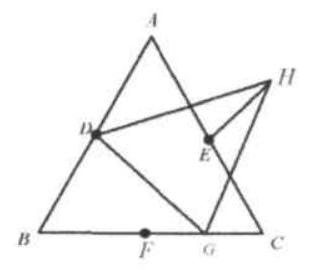
\includegraphics[width=\textwidth]{images/045(3).jpg}

\section*{Solution}
Connect \(D E, D F\).\\
Since \(\triangle A B C\) is an equilateral triangle, \(D E=\frac{1}{2} B C=\frac{1}{2} A C=D F\).\\
\(D E / / B C, D F / / A C\).\\
\(\angle E D F=\angle A C B=60^{\circ}\).\\
\centering
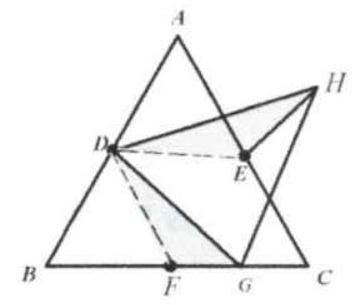
\includegraphics[width=\textwidth]{images/051(2).jpg}

Since \(\triangle D G H\) is an equilateral triangle, \(D H=D G, \angle H D G=60^{\circ}\).\\
Thus \(\angle F D G=60^{\circ}-\angle G D E=\angle E D H\).\\
So \(\triangle F D G \cong \triangle E D H\). \(F G=E H\).

\end{document}
